\documentclass[../monografia.tex]{subfiles}

\begin{document}
\section{Motivação}

Com o aumento do tempo que as pessoas passam em ambientes fechados, como escritórios, há um crescente interesse em monitorar e controlar tais ambientes, visando uma melhora na saúde e conforto das pessoas, impactando a qualidade de vida e até a produtividade. Espaços que implementam essas soluções são comumente chamados de prédios inteligentes (\textit{smart buildings}, do inglês). É possível até mesmo que esse controle seja utilizado para uma atuação de maneira energeticamente sustentável e, dentro desse contexto, surgem os \textit{green buildings} (em português, construções sustentáveis) \cite{GreenBuildings} \cite{EnergyBuildings}.

No desenvolvimento de construções civis sustentáveis, torna-se necessário que seja pensada a implementação automatizada deste monitoramento dos ambientes desde o projeto da edificação e sua concepção, ocorrendo de forma integrada à construção. Uma pesquisa mais aprofundada sobre o conforto dos ambientes pode interferir no projeto, de modo que sejam repensados materiais utilizados e sistemas de aquecimento, ventilação, iluminação, dentre outros. Assim como a sua implementação, pesquisas na área de conforto têm se tornado cada vez mais importantes. 

%Proposta
Foi com essa necessidade e a proposta de desenvolver um dispositivo eletrônico que o professor Vanderley M. John, do departamento de Construção Civil da Poli (PCC) e coordenador do CICS (Centro de Inovação em Construção Sustentável da USP) \cite{CICS}, entrou em contato conosco. A fim de viabilizar o estudo de qualidade e conforto em ambientes internos (ou IEQ, do inglês \textit{Indoor Environmental Quality}), faz-se necessária a medição de diversos indicadores no ambiente e uma coleta periódica da opinião das pessoas, atrelada às medições quantitativas para que, dessa forma, seja possível identificar como uma afeta a outra. 

Podemos elencar 4 parâmetros principais que metrificam a qualidade de ambientes, sendo eles qualidade térmica, luminosa, olfativa (qualidade do ar) e acústica. Estudos e soluções presentes no mercado que abordam a coleta de parâmetros de ambientes fechados, em sua maioria, são focados em monitorar apenas alguns desses indicadores, discutidos no capítulo \ref{cap:arte} deste trabalho, além de poucos apresentarem um esforço em observar a real percepção de conforto das pessoas que ocupam tal local e correlacioná-la com os dados medidos.

O desenvolvimento de um dispositivo embarcado tem, portanto, além de uma aplicação prática monitorando a qualidade para as pessoas, também grande utilidade em pesquisas de construção civil e arquitetura, com medições mais precisas e incluindo um elemento muitas vezes deixado de lado: o fator humano.

Em edifícios, escritórios são hoje os que ocupam a maior área física e tem o maior consumo de energia, sendo sistemas de iluminação, aquecimento e resfriamento (como ar condicionado) os principais causadores do alto consumo \cite{EnergyBuildings}. Por isso, escritórios são o nicho escolhido para o estudo de conforto pelo departamento PCC e, consequentemente, para a implementação dessa rede de dispositivos. 


\section{Objetivos}

O objetivo deste trabalho é o projeto de uma rede de dispositivos sensoreados que viabiliza o estudo de qualidade e conforto em escritórios, fazendo coletas de ao menos uma informação relativa aos principais indicadores de qualidade do ambiente. Para uma cobertura completa de grandes escritórios é importante que existam diversos dispositivos espalhados, conectados em rede. Esse grande volume de dados coletados será salvo em um banco de dados e apresentado de forma gráfica em uma plataforma para facilitar a interpretação e análise durante sua aplicação, como ferramenta de estudo. 

%dispositivos
Além da coleta de dados que remetem à qualidade geral do local estudado, propõe-se também que cada dispositivo seja capaz de fazer a coleta de \textit{feedback} dos ocupantes através de uma interface no próprio dispositivo com perguntas que abordam o estado atual do ambiente, sendo necessário que os dispositivos estejam próximos à pessoa da qual serão coletadas as opiniões relativas ao conforto para que seja possível relacionar dados medidos pelos sensores com o conforto percebido pelas pessoas.

% Viabilizando o estudo, estes parâmetros a serem coletados podem ser iterados, aumentando ou alterando as informações, conforme a pesquisa avança. Com um projeto \textit{open source} é possível fazer alterações neste ou integrá-lo a outros dispositivos disponíveis no mercado para esse fim. 


\section{Árvore de Objetivos} 
% arvore de objetivos
A árvore de objetivos é uma representação gráfica dos meios necessários, chamados objetivos específicos, para alcançar o objetivo geral do projeto. 
Para atingir o objetivo geral do projeto, que é a realização de uma rede de dispositivos, com monitoramento do ambiente e apresentação dos dados, a seguinte árvore de objetivos foi elaborada, com a porcentagem de dedicação ao lado de cada um.

\begin{figure}[h!]
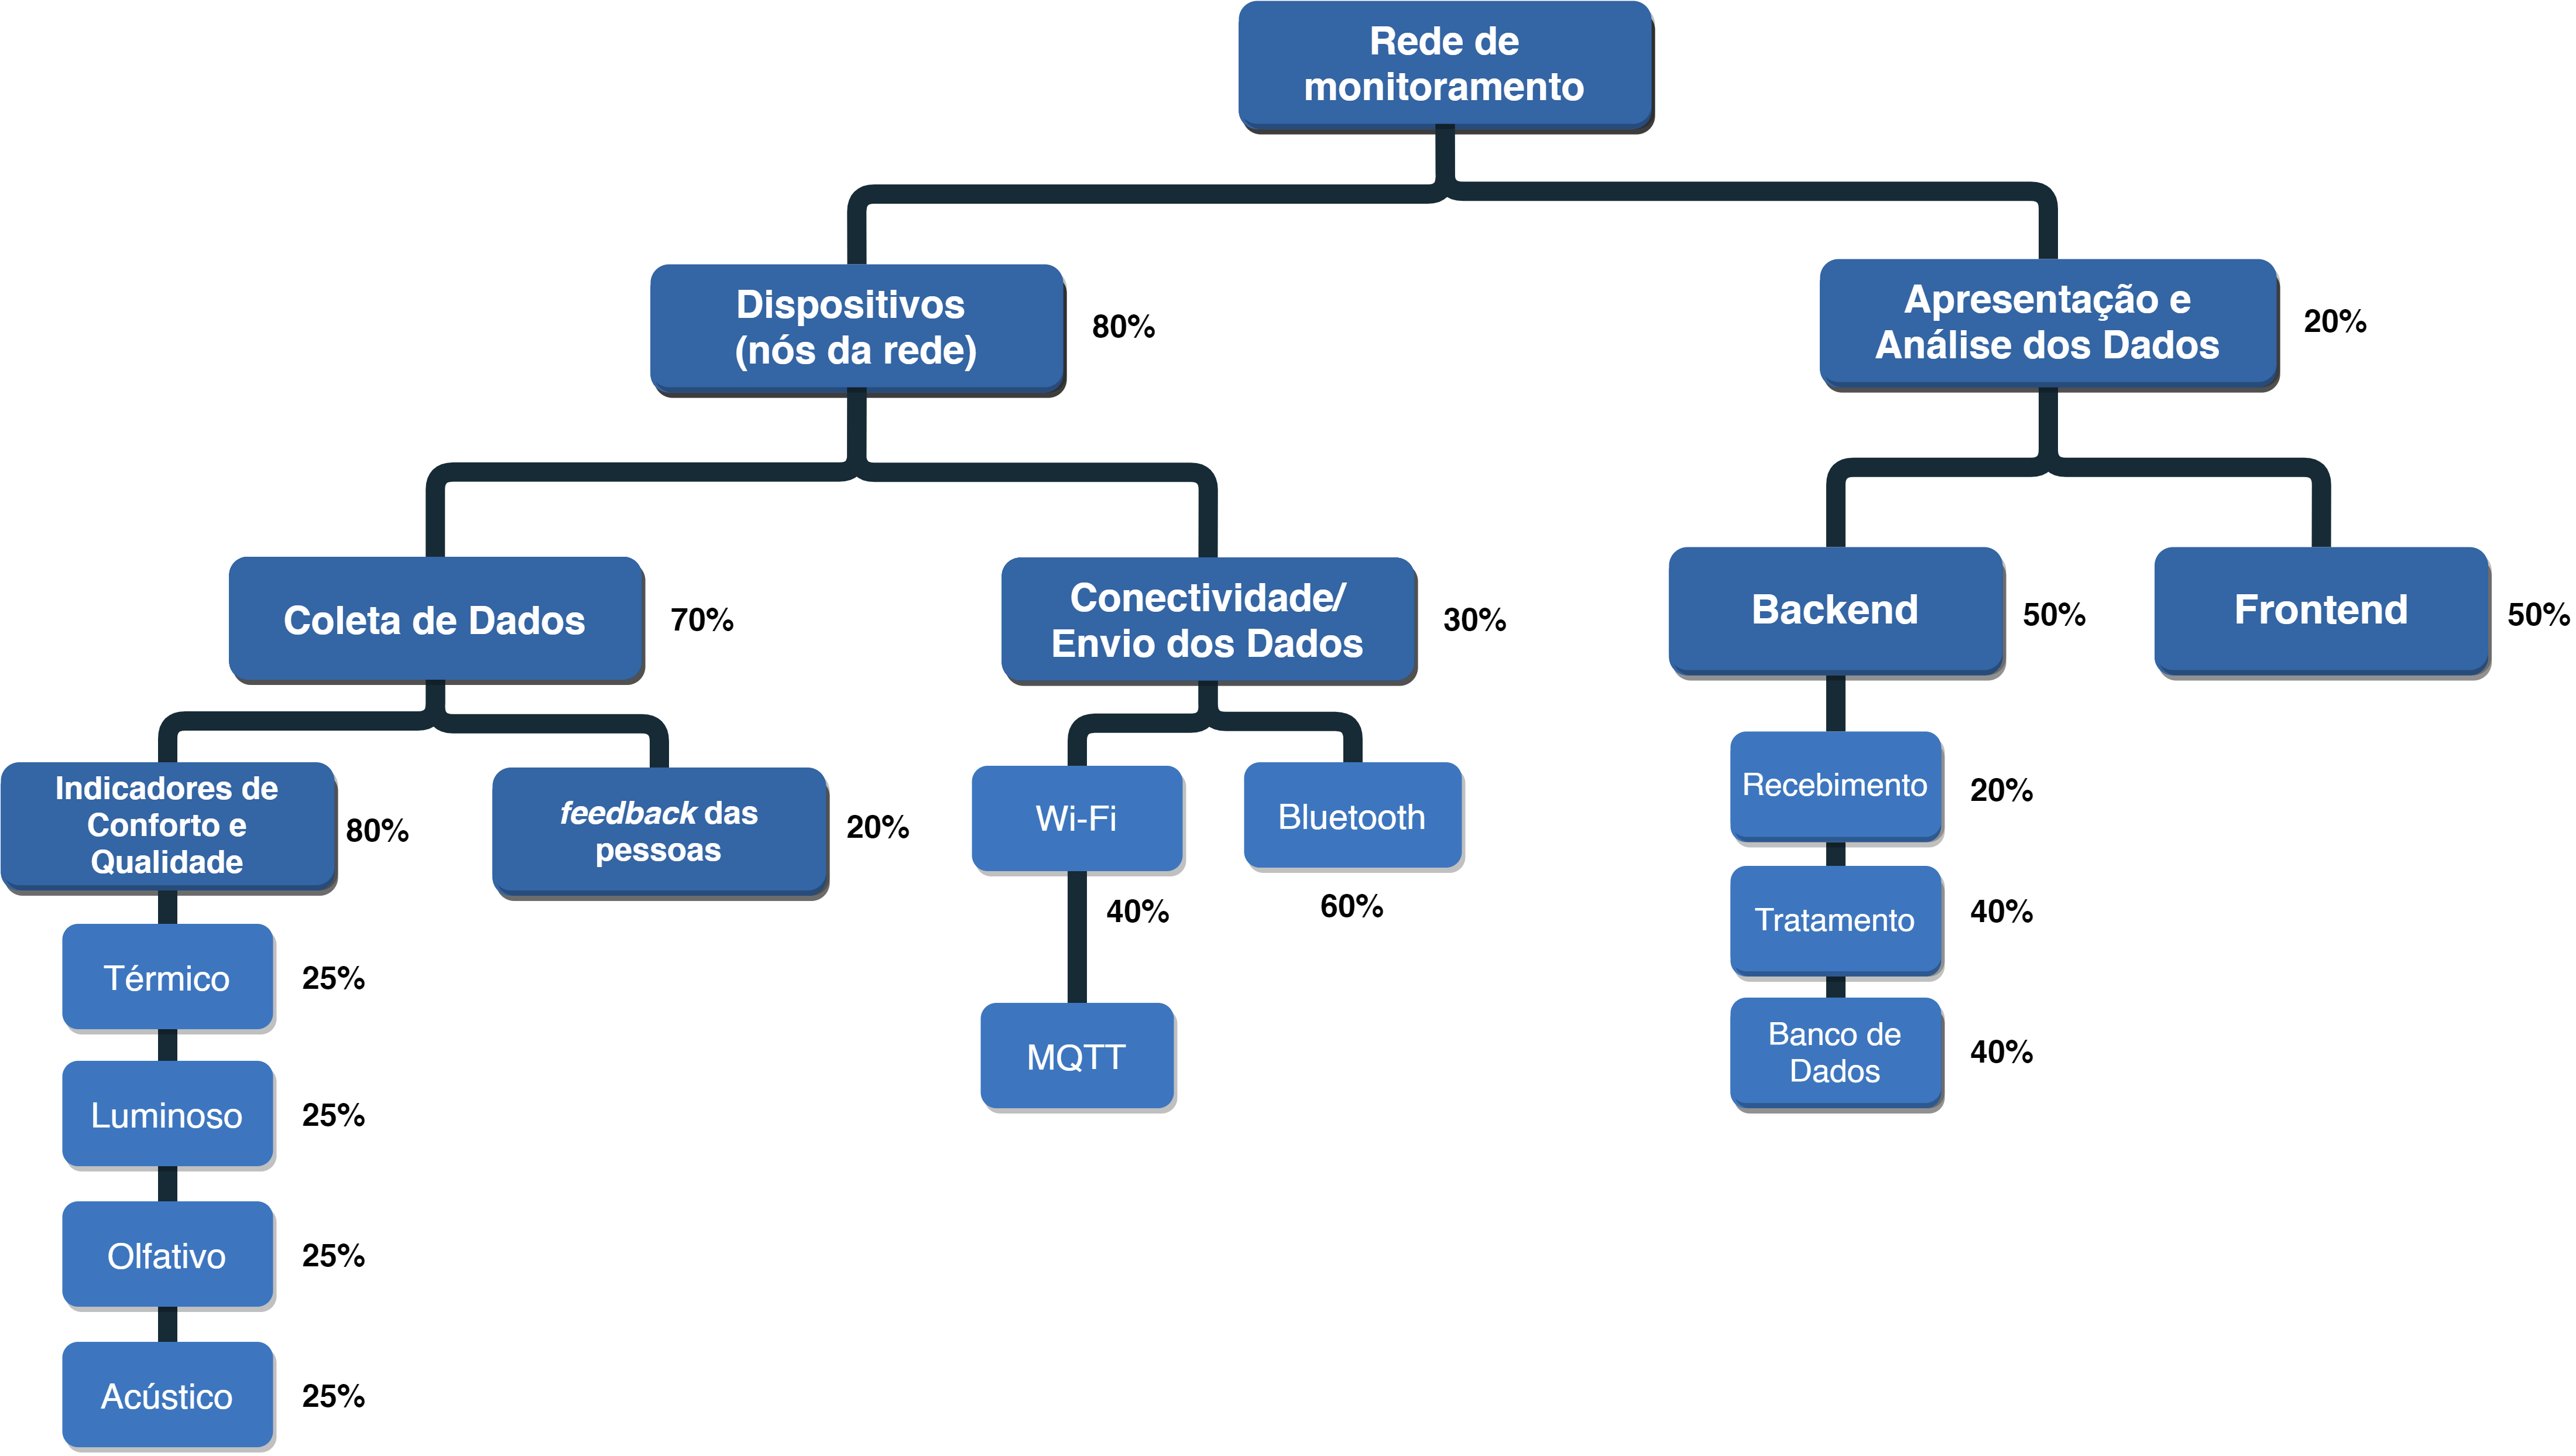
\includegraphics[scale=0.1]{arvore_de_objetivos}
\centering
\caption{Árvore de objetivos do projeto.}
\label{fig:objective-tree}
\end{figure}

\end{document}